% questions.tex —— 2003 年·全国旧课程卷·理科 · 题目内容片段（无答案）
% 由 tools/generate_projects.py 依来源总账自 2003/2003_数学真题_全国旧课程理_试题.md 生成，勿手改（改源 MD 后重跑）


\gkpart{数学}

\begin{gktip}
\textbf{来源说明}：本题面依据固定源 PDF 两页 A3 题面逐题转录，原卷印刷页码 134–135。固定源不附答案，答案和解析均由本库独立复算。

\textbf{图形说明}：第 15、16、18、20、21 题的原卷图形关系重绘为 TikZ/PGFPlots 矢量图。图形标记所指的 PNG 不随仓库保存。
\end{gktip}

\gkpart{一、选择题}

\begin{question}
\gkti{1}已知 $x\in\left(-\dfrac\pi2,0\right)$，$\cos x=\dfrac45$，则 $\tan2x=$\mbox{（　　）}

（A）$\dfrac7{24}$　　（B）$-\dfrac7{24}$　　（C）$\dfrac{24}{7}$　　（D）$-\dfrac{24}{7}$

\end{question}
\begin{question}
\gkti{2}圆锥曲线

\nopagebreak[4]
\[
\rho=\frac{8\sin\theta}{\cos^2\theta}
\]

的准线方程是\mbox{（　　）}

（A）$\rho\cos\theta=-2$　　（B）$\rho\cos\theta=2$　　（C）$\rho\sin\theta=2$　　（D）$\rho\sin\theta=-2$

\end{question}
\begin{question}
\gkti{3}设函数

\nopagebreak[4]
\[
f(x)=
\begin{cases}
2^{-x}-1,&x\leqslant0,\\
x^2,&x>0,
\end{cases}
\]

若 $f(x_0)>1$，则 $x_0$ 的取值范围是\mbox{（　　）}

（A）$(-1,1)$　　（B）$(-1,+\infty)$

（C）$(-\infty,-2)\cup(0,+\infty)$　　（D）$(-\infty,-1)\cup(1,+\infty)$

\end{question}
\begin{question}
\gkti{4}函数 $y=2\sin x(\sin x+\cos x)$ 的最大值为\mbox{（　　）}

（A）$1+\sqrt2$　　（B）$\sqrt2-1$　　（C）$\sqrt2$　　（D）$2$

\end{question}
\begin{question}
\gkti{5}已知圆 $C:(x-a)^2+(y-2)^2=4$（$a>0$）及直线 $l:x-y+3=0$，当直线 $l$ 被 $C$ 截得的弦长为 $2\sqrt3$ 时，$a$ 的值等于\mbox{（　　）}

（A）$\sqrt2$　　（B）$2-\sqrt2$　　（C）$\sqrt2-1$　　（D）$\sqrt2+1$

\end{question}
\begin{question}
\gkti{6}已知圆锥的底面半径为 $R$、高为 $3R$，在它的所有内接圆柱中，全面积的最大值是\mbox{（　　）}

（A）$2\pi R^2$　　（B）$\dfrac94\pi R^2$　　（C）$\dfrac83\pi R^2$　　（D）$\dfrac32\pi R^2$

\end{question}
\begin{question}
\gkti{7}已知方程

\nopagebreak[4]
\[
(x^2-2x+m)(x^2-2x+n)=0
\]

的四个根组成一个首项为 $\dfrac14$ 的等差数列，则 $|m-n|=$\mbox{（　　）}

（A）$1$　　（B）$\dfrac34$　　（C）$\dfrac12$　　（D）$\dfrac38$

\end{question}
\begin{question}
\gkti{8}已知双曲线中心在原点且一个焦点为 $F(\sqrt7,0)$，直线 $y=x-1$ 与其相交于 $M\text{、}N$ 两点，$MN$ 中点的横坐标为 $-\dfrac23$，则此双曲线的方程是\mbox{（　　）}

（A）$\dfrac{x^2}{3}-\dfrac{y^2}{4}=1$　　（B）$\dfrac{x^2}{4}-\dfrac{y^2}{3}=1$

（C）$\dfrac{x^2}{5}-\dfrac{y^2}{2}=1$　　（D）$\dfrac{x^2}{2}-\dfrac{y^2}{5}=1$

\end{question}
\begin{question}
\gkti{9}函数 $f(x)=\sin x$，$x\in\left[\dfrac\pi2,\dfrac{3\pi}2\right]$ 的反函数 $f^{-1}(x)=$\mbox{（　　）}

（A）$-\arcsin x,\ x\in[-1,1]$　　（B）$-\pi-\arcsin x,\ x\in[-1,1]$

（C）$\pi+\arcsin x,\ x\in[-1,1]$　　（D）$\pi-\arcsin x,\ x\in[-1,1]$

\end{question}
\begin{question}
\gkti{10}已知长方形的四个顶点 $A(0,0)\text{、}B(2,0)\text{、}C(2,1)\text{、}D(0,1)$，一质点从 $AB$ 的中点 $P_0$ 沿与 $AB$ 的夹角为 $\theta$ 的方向射到 $BC$ 上的点 $P_1$ 后，依次反射到 $CD\text{、}DA$ 和 $AB$ 上的点 $P_2\text{、}P_3$ 和 $P_4$（入射角等于反射角）。设 $P_4$ 的坐标为 $(x_4,0)$，若 $1<x_4<2$，则 $\tan\theta$ 的取值范围是\mbox{（　　）}

（A）$\left(\dfrac13,1\right)$　　（B）$\left(\dfrac13,\dfrac23\right)$　　（C）$\left(\dfrac25,\dfrac12\right)$　　（D）$\left(\dfrac25,\dfrac23\right)$

\end{question}
\begin{question}
\gkti{11}

\nopagebreak[4]
\[
\lim_{n\to\infty}
\frac{C_2^2+C_3^2+C_4^2+\cdots+C_n^2}
n(C_2^1+C_3^1+C_4^1+\cdots+C_n^1)
\]

的值为\mbox{（　　）}

（A）$3$　　（B）$\dfrac13$　　（C）$\dfrac16$　　（D）$6$

\end{question}
\begin{question}
\gkti{12}一个四面体的所有棱长都为 $\sqrt2$，四个顶点在同一球面上，则此球的表面积为\mbox{（　　）}

（A）$3\pi$　　（B）$4\pi$　　（C）$3\sqrt3\pi$　　（D）$6\pi$

\end{question}
\gkpart{二、填空题}

\begin{question}
\gkti{13}$\left(x^2-\dfrac1{2x}\right)^9$ 的展开式中 $x^9$ 的系数是\gkblank{}。

\end{question}
\begin{question}
\gkti{14}使 $\log_2(-x)<x+1$ 成立的 $x$ 的取值范围是\gkblank{}。

\Needspace{0.4\textheight}
\end{question}
\begin{question}
\gkti{15}如图，一个地区分为 5 个行政区域，现给地图着色，要求相邻地区不得使用同一颜色，现有 4 种颜色可供选择，则不同的着色方法共有\gkblank{}种。（以数字作答）
\nopagebreak[4]
\begin{center}% 2003 年全国旧课程理科第 15 题：行政区域着色图
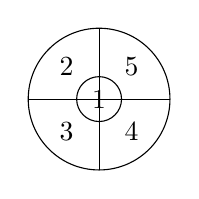
\begin{tikzpicture}[scale=0.75]
  \draw (0,0) circle (1.2);
  \draw (0,-1.2)--(0,1.2) (-1.2,0)--(1.2,0);
  \draw (0,0) circle (0.38);
  \node at (0,0) {1};
  \node at (-0.55,0.55) {2};
  \node at (0.55,0.55) {5};
  \node at (-0.55,-0.55) {3};
  \node at (0.55,-0.55) {4};
\end{tikzpicture}
\end{center}
\nopagebreak[4]
\Needspace{0.4\textheight}
\end{question}
\begin{question}
\gkti{16}下列 5 个正方体图形中，$l$ 是正方体的一条对角线，点 $M\text{、}N\text{、}P$ 分别为其所在棱的中点，能得出 $l\perp$ 面 $MNP$ 的图形的序号是\gkblank{}。（写出所有符合要求的图形序号）
\nopagebreak[4]
\begin{center}% 2003 年全国旧课程理科第 16 题：正方体选项示意
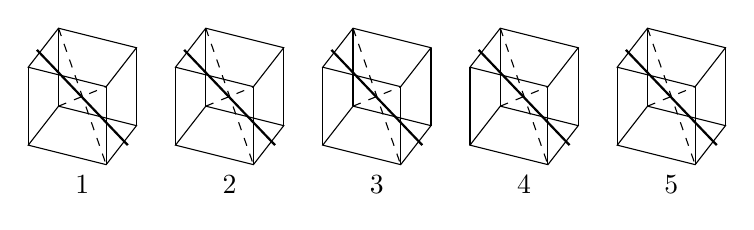
\begin{tikzpicture}[>=stealth,scale=0.55]
  \foreach \sx/\lab in {0/1,3.4/2,6.8/3,10.2/4,13.6/5}
  {
    \begin{scope}[shift={(\sx,0)}]
      \draw (0,0)--(1.8,-0.45)--(2.5,0.45)--(0.7,0.9)--cycle;
      \draw (0,0)--(0,1.8) (1.8,-0.45)--(1.8,1.35)
        (2.5,0.45)--(2.5,2.25) (0.7,0.9)--(0.7,2.7);
      \draw (0,1.8)--(1.8,1.35)--(2.5,2.25)--(0.7,2.7)--cycle;
      \draw[dashed] (0.7,0.9)--(1.8,1.35) (0.7,2.7)--(1.8,-0.45);
      \draw[thick] (0.2,2.2)--(2.3,0.0);
      \node at (1.25,-0.9) {\lab};
    \end{scope}
  }
\end{tikzpicture}
\end{center}
\nopagebreak[4]
\end{question}
\gkpart{三、解答题}

\begin{question}
\gkti{17}已知复数 $z$ 的辐角为 $60^\circ$，且 $|z-1|$ 是 $|z|$ 和 $|z-2|$ 的等比中项，求 $|z|$。

\Needspace{0.4\textheight}
\end{question}
\begin{question}
\gkti{18}如图，在直三棱柱 $ABC-A_1B_1C_1$ 中，底面是等腰直角三角形，$\angle ACB=90^\circ$，侧棱 $AA_1=2$，$D\text{、}E$ 分别是 $CC_1$ 与 $A_1B$ 的中点，点 $E$ 在平面 $ABD$ 上的射影是 $\triangle ABD$ 的重心 $G$。
\nopagebreak[4]
\begin{center}% 2003 年全国旧课程理科第 18 题：直三棱柱
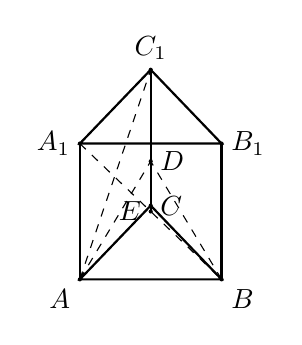
\begin{tikzpicture}[>=stealth,scale=0.75]
  \coordinate (A) at (0,0); \coordinate (B) at (2.4,0);
  \coordinate (C) at (1.2,1.25); \coordinate (A1) at (0,2.3);
  \coordinate (B1) at (2.4,2.3); \coordinate (C1) at (1.2,3.55);
  \coordinate (D) at (1.2,2.0); \coordinate (E) at (1.2,1.15);
  \draw[thick] (A)--(B)--(C)--cycle;
  \draw[thick] (A1)--(B1)--(C1)--cycle;
  \draw[thick] (A)--(A1) (B)--(B1) (C)--(C1);
  \draw[dashed] (A1)--(B) (A)--(C1) (A)--(D) (B)--(D);
  \draw[thick] (E)--(D);
  \fill (A) circle (1pt) node[below left] {$A$};
  \fill (B) circle (1pt) node[below right] {$B$};
  \fill (C) circle (1pt) node[right] {$C$};
  \fill (A1) circle (1pt) node[left] {$A_1$};
  \fill (B1) circle (1pt) node[right] {$B_1$};
  \fill (C1) circle (1pt) node[above] {$C_1$};
  \fill (D) circle (1pt) node[right] {$D$};
  \fill (E) circle (1pt) node[left] {$E$};
\end{tikzpicture}
\end{center}
\nopagebreak[4]
（1） 求 $A_1B$ 与平面 $ABD$ 所成角的大小（结果用反三角函数值表示）；

（2） 求点 $A_1$ 到平面 $AED$ 的距离。

\end{question}
\begin{question}
\gkti{19}已知 $c>0$，设

\nopagebreak[4]
\[
P:\text{\text{函数} }y=c^x\text{ \text{在} }\mathbb R\text{ \text{上单调递减}};
\qquad
Q:\text{\text{不等式} }x+|x-2c|>1\text{ \text{的解集为} }\mathbb R.
\]

如果 $P$ 和 $Q$ 有且仅有一个正确，求 $c$ 的取值范围。

\Needspace{0.4\textheight}
\end{question}
\begin{question}
\gkti{20}在某海滨城市附近海面有一台风。据监测，当前台风中心位于城市 $O$（如图）的东偏南 $\theta$ 方向 300 km 的海面 $P$ 处，并以 20 km/h 的速度向西偏北 $45^\circ$ 方向移动，台风侵袭的范围为圆形区域，当前半径为 60 km，并以 10 km/h 的速度不断增大，问几小时后该城市开始受到台风的侵袭？
\nopagebreak[4]
\begin{center}% 2003 年全国旧课程理科第 20 题：台风运动示意图
\begin{tikzpicture}[>=stealth,scale=0.72]
  \draw[->] (-2.8,0)--(3.2,0) node[right] {东};
  \draw[->] (0,-2.3)--(0,2.5) node[above] {北};
  \fill (0,0) circle (1.5pt) node[below left] {$O$};
  \fill (-1.8,-1.25) circle (1.5pt) node[below] {$P$};
  \draw[->,thick] (-1.8,-1.25)--(0.2,0.75) node[midway,below] {$20$ km/h};
  \draw[dashed] (-1.8,-1.25) circle (0.55);
  \node at (-1.35,-1.75) {$r(t)$};
\end{tikzpicture}
\end{center}
\nopagebreak[4]
\Needspace{0.4\textheight}
\end{question}
\begin{question}
\gkti{21}已知常数 $a>0$，在矩形 $ABCD$ 中，$AB=4$，$BC=4a$，$O$ 为 $AB$ 的中点，点 $E\text{、}F\text{、}G$ 分别在 $BC\text{、}CD\text{、}DA$ 上移动，且

\nopagebreak[4]
\[
\frac{BE}{BC}=\frac{CF}{CD}=\frac{DG}{DA},
\]

$P$ 为 $GE$ 与 $OF$ 的交点（如图）。问是否存在两个定点，使 $P$ 到这两点的距离之和为定值？若存在，求出这两点的坐标及此定值；若不存在，请说明理由。
\nopagebreak[4]
\begin{center}% 2003 年全国旧课程理科第 21 题：矩形动点示意图
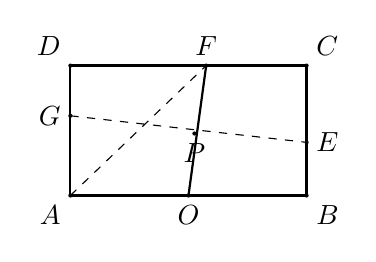
\begin{tikzpicture}[>=stealth,scale=0.75]
  \coordinate (A) at (0,0); \coordinate (B) at (4,0);
  \coordinate (C) at (4,2.2); \coordinate (D) at (0,2.2);
  \coordinate (E) at (4,0.9); \coordinate (F) at (2.3,2.2);
  \coordinate (G) at (0,1.35); \coordinate (P) at (2.1,1.05);
  \coordinate (O) at (2,0);
  \draw[thick] (A)--(B)--(C)--(D)--cycle;
  \draw[dashed] (G)--(E) (A)--(F);
  \draw[thick] (O)--(F);
  \fill (A) circle (1pt) node[below left] {$A$};
  \fill (B) circle (1pt) node[below right] {$B$};
  \fill (C) circle (1pt) node[above right] {$C$};
  \fill (D) circle (1pt) node[above left] {$D$};
  \fill (E) circle (1pt) node[right] {$E$};
  \fill (F) circle (1pt) node[above] {$F$};
  \fill (G) circle (1pt) node[left] {$G$};
  \fill (P) circle (1pt) node[below] {$P$};
  \fill (O) circle (1pt) node[below] {$O$};
\end{tikzpicture}
\end{center}
\nopagebreak[4]
\end{question}
\begin{question}
\gkti{22}【甲】设 $\{a_n\}$ 是集合

\nopagebreak[4]
\[
\{2^s+2^t\mid 0\leqslant s<t,\ s,t\in\mathbb Z\}
\]

\Needspace{5\baselineskip}
中所有的数从小到大排列成的数列，即 $a_1=3\text{、}a_2=5\text{、}a_3=6\text{、}a_4=9\text{、}a_5=10\text{、}a_6=12\text{、}\ldots$。将数列 $\{a_n\}$ 各项按照“上小下大，左小右大”的原则写成三角形数表：

\nopagebreak[4]
\[
\begin{array}{c}
3\\
5\quad6\\
9\quad10\quad12\\
\cdots
\end{array}
\]

（1） 写出这个三角形数表的第四行、第五行各数；

（2） 求 $a_{100}$。

\Needspace{5\baselineskip}
（3） 【乙】设 $\{b_n\}$ 是集合

\nopagebreak[4]
\[
\{2^r+2^s+2^t\mid 0\leqslant r<s<t,\ r,s,t\in\mathbb Z\}
\]

中所有的数从小到大排列成的数列，已知 $b_k=1160$，求 $k$。

\end{question}